% ============================================================
% CHƯƠNG 2: KIẾN THỨC NỀN TẢNG
% ============================================================

\chapter{Kiến thức nền tảng}

\section{Tổng quan về kiến trúc hệ thống}

Hệ thống SmartNutri được thiết kế theo mô hình \textbf{ba tầng} (three-tier architecture), tách biệt rõ trách nhiệm giữa giao diện, logic xử lý và lưu trữ dữ liệu.

\subsection{Tầng trình bày (Presentation Tier)}

Tầng trình bày gồm hai thành phần chính:

\begin{itemize}
    \item \textbf{Ứng dụng di động Flutter:} Là giao diện chính cho người dùng cuối, cung cấp các màn hình đăng ký/đăng nhập, onboarding, trang chủ, nhật ký ăn uống, quét món ăn, thống kê dinh dưỡng, chatbot AI và quản lý hồ sơ. Ứng dụng giao tiếp trực tiếp với Firebase Authentication và Firestore thông qua Firebase SDK, sử dụng Provider/ChangeNotifier để quản lý trạng thái và cập nhật UI khi dữ liệu thay đổi.
    \item \textbf{Trang quản trị web (React + TypeScript + Vite):} Dành cho quản trị viên, cung cấp giao diện quản lý cơ sở dữ liệu thực phẩm (thêm, sửa, xóa, import CSV) và quản lý người dùng (phân quyền admin, gán gói Premium). Trang admin giao tiếp với Firestore và Cloud Functions thông qua Firebase Web SDK.
\end{itemize}

\subsection{Tầng ứng dụng (Application Tier)}

Tầng ứng dụng bao gồm Firebase Cloud Functions và Google Gemini API, đảm nhận các tác vụ yêu cầu xử lý phía máy chủ:

\begin{itemize}
    \item \textbf{Firebase Cloud Functions:} Đóng vai trò là tầng logic trung gian giữa client và các dịch vụ bên ngoài. Các nghiệp vụ backend như nhận diện món ăn bằng AI, gợi ý bữa ăn, phân quyền người dùng và import dữ liệu được đóng gói trong các Cloud Function riêng biệt, gọi được từ cả ứng dụng di động lẫn trang admin thông qua HTTP request có kèm token xác thực.
    \item \textbf{Google Gemini API:} Được gọi từ phía Cloud Functions (không gọi trực tiếp từ client) để thực hiện nhận diện món ăn từ ảnh và trả lời câu hỏi tư vấn dinh dưỡng. Việc gọi Gemini qua Cloud Functions giúp bảo vệ API key — khóa được lưu dưới dạng biến môi trường trên Cloud Functions và không bao giờ xuất hiện trong mã nguồn phía client.
    \item \textbf{Firebase Authentication:} Xử lý xác thực người dùng (email/password và Google Sign-In), quản lý phiên đăng nhập và cấp token để xác định danh tính người dùng trong các request đến Firestore và Cloud Functions.
\end{itemize}

\subsection{Tầng dữ liệu (Data Tier)}

Tầng dữ liệu được xây dựng trên hai dịch vụ của Firebase:

\begin{itemize}
    \item \textbf{Cloud Firestore:} Cơ sở dữ liệu NoSQL dạng document, lưu trữ toàn bộ dữ liệu của hệ thống. Các collection chính gồm: \texttt{users} (thông tin tài khoản, subscription, aiScanUsage), \texttt{foods} (danh mục thực phẩm), và các subcollection như \texttt{users/\{uid\}/meal\_entries} (nhật ký ăn uống), \texttt{users/\{uid\}/favorites} (món yêu thích), \texttt{users/\{uid\}/usage} (quota quét AI theo tháng), \texttt{users/\{uid\}/chat\_history} (lịch sử trò chuyện với AI). Dữ liệu được phân tách theo UID, đảm bảo mỗi người dùng chỉ truy cập được dữ liệu của chính mình thông qua Firestore Security Rules.
    \item \textbf{Firebase Storage:} Lưu trữ file tĩnh, chủ yếu là ảnh đại diện người dùng và ảnh món ăn tải lên trong quá trình quét AI, được tổ chức theo đường dẫn \texttt{users/\{uid\}/}.
\end{itemize}

\begin{figure}[H]
    \centering
    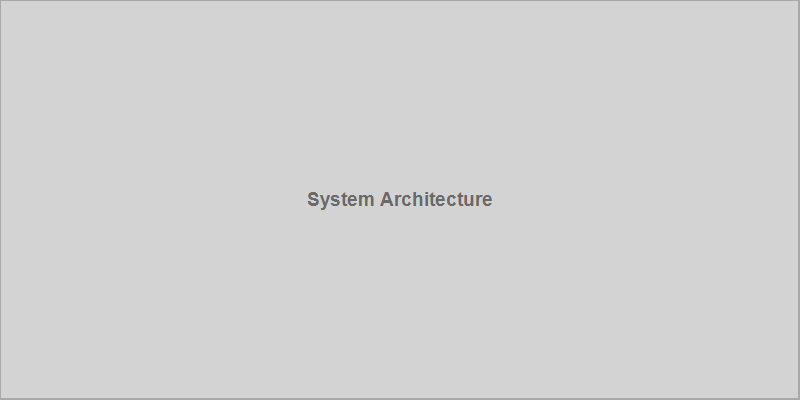
\includegraphics[width=0.85\textwidth]{assets/diagrams/system_architecture.png}
    \caption{Kiến trúc tổng thể hệ thống SmartNutri}
    \label{fig:system_architecture}
\end{figure}

\subsection{Luồng xử lý quét món ăn bằng AI}

Để minh họa cách các tầng phối hợp với nhau, dưới đây là luồng xử lý của tính năng quét món ăn — một trong những chức năng cốt lõi của hệ thống:

\begin{enumerate}
    \item Người dùng chụp hoặc chọn ảnh món ăn từ ứng dụng Flutter (tầng trình bày).
    \item Ảnh được resize và chuyển thành chuỗi base64, sau đó gửi đến Cloud Function \texttt{identifyFoodImage} qua HTTP request kèm Firebase Auth token.
    \item Cloud Function (tầng ứng dụng) xác thực token, kiểm tra quota quét AI của người dùng trong Firestore (tầng dữ liệu). Nếu người dùng gói free đã hết lượt quét trong tháng, Cloud Function từ chối yêu cầu và trả về lỗi.
    \item Nếu còn quota, Cloud Function gửi ảnh kèm prompt phân tích đến Gemini API. Prompt được thiết kế để Gemini trả về danh sách món ăn dưới dạng JSON có cấu trúc, bao gồm tên món, calo ước tính, protein, carbohydrate, chất béo, khối lượng phần ăn và độ tự tin.
    \item Gemini API trả về kết quả cho Cloud Function. Cloud Function cập nhật số lượt quét đã sử dụng trong Firestore, sau đó trả kết quả về ứng dụng.
    \item Ứng dụng hiển thị kết quả cho người dùng. Người dùng có thể xác nhận để thêm món ăn vào nhật ký (lưu vào subcollection \texttt{meal\_entries} trong Firestore) hoặc chỉnh sửa thông tin dinh dưỡng trước khi lưu.
\end{enumerate}

\subsection{Cơ chế giao tiếp giữa các tầng}

Hệ thống sử dụng hai cơ chế giao tiếp chính:

\begin{itemize}
    \item \textbf{Firebase SDK (trực tiếp):} Ứng dụng Flutter và trang admin giao tiếp trực tiếp với Firestore, Storage và Authentication thông qua Firebase SDK. Đây là cơ chế chính cho hầu hết các thao tác đọc/ghi dữ liệu người dùng.
    \item \textbf{Cloud Functions (HTTP request):} Các tác vụ cần xử lý phía máy chủ hoặc gọi dịch vụ bên ngoài (như Gemini API) được đóng gói trong Cloud Function và gọi qua HTTP request có kèm token xác thực Firebase.
\end{itemize}

Trong ứng dụng Flutter, code được tổ chức theo cấu trúc \textbf{feature-first}: mỗi tính năng (đăng nhập, nhật ký ăn uống, quét món ăn, chatbot,\ldots) được đặt trong một thư mục riêng, gồm hai tầng con là \textit{domain} (model, service) và \textit{presentation} (widget, page).

\section{Các công nghệ được sử dụng}

\subsection{Firebase}

Firebase là nền tảng phát triển ứng dụng của Google, cung cấp các dịch vụ backend dưới dạng BaaS (Backend-as-a-Service). SmartNutri lựa chọn Firebase làm nền tảng backend chính vì khả năng tích hợp sẵn giữa các dịch vụ và mô hình lập trình phía client, giúp nhóm phát triển tập trung vào logic nghiệp vụ thay vì quản lý hạ tầng máy chủ.

\subsubsection{Firebase Authentication}

Firebase Authentication \cite{firebase_auth} cung cấp hệ thống xác thực người dùng với nhiều phương thức đăng nhập. Trong SmartNutri, dịch vụ này được sử dụng để:

\begin{itemize}
    \item Cho phép người dùng đăng ký và đăng nhập bằng email/mật khẩu.
    \item Hỗ trợ đăng nhập nhanh qua tài khoản Google.
    \item Tự động quản lý phiên đăng nhập và refresh token, đảm bảo người dùng không phải đăng nhập lại mỗi lần mở ứng dụng.
\end{itemize}

Mỗi người dùng sau khi xác thực được gán một mã định danh duy nhất (UID), mã này được dùng làm khóa chính cho toàn bộ dữ liệu cá nhân trong Firestore, đảm bảo dữ liệu được phân tách rõ ràng giữa những người dùng khác nhau.

\subsubsection{Cloud Firestore}

Cloud Firestore \cite{firebase_firestore} là cơ sở dữ liệu NoSQL dạng document của Firebase. Dữ liệu được tổ chức thành các collection, mỗi collection chứa nhiều document — mỗi document là một bản ghi JSON linh hoạt, không yêu cầu schema cố định. Firestore được chọn cho SmartNutri vì các lý do sau:

\begin{itemize}
    \item \textbf{Cấu trúc dữ liệu theo từng người dùng:} Mô hình subcollection của Firestore (ví dụ: \texttt{users/\{uid\}/meal\_entries/\{entryId\}}) cho phép tổ chức dữ liệu nhật ký ăn uống, món yêu thích, lịch sử chat của từng người dùng một cách tự nhiên và hiệu quả.
    \item \textbf{Đồng bộ thời gian thực:} Khi người dùng thêm một món ăn vào nhật ký, dữ liệu được cập nhật ngay lập tức trên giao diện mà không cần thao tác làm mới thủ công, nhờ cơ chế snapshot listener của Firestore.
    \item \textbf{Security Rules:} Cho phép định nghĩa quy tắc bảo mật trực tiếp trên Firestore, đảm bảo mỗi người dùng chỉ có thể đọc và ghi dữ liệu thuộc về chính mình.
    \item \textbf{Hỗ trợ offline:} Firestore tự động lưu đệm dữ liệu trên thiết bị, cho phép ứng dụng hoạt động ngay cả khi không có kết nối mạng và tự động đồng bộ khi kết nối được khôi phục.
\end{itemize}

\subsubsection{Firebase Storage}

Firebase Storage \cite{firebase_storage} cung cấp dịch vụ lưu trữ file trên đám mây, tích hợp với Firebase Authentication để kiểm soát quyền truy cập. Trong SmartNutri, Storage được sử dụng để lưu trữ ảnh đại diện (avatar) của người dùng và ảnh món ăn do người dùng tải lên trong quá trình sử dụng tính năng quét AI. Các file được tổ chức theo cấu trúc thư mục \texttt{users/\{uid\}/} để đảm bảo mỗi người dùng chỉ truy cập được file của chính mình.

\subsubsection{Firebase Cloud Functions}

Cloud Functions \cite{firebase_functions} là môi trường serverless cho phép chạy code backend mà không cần quản lý máy chủ. Trong SmartNutri, Cloud Functions đảm nhận các tác vụ không nên thực hiện trực tiếp từ phía client:

\begin{itemize}
    \item \textbf{Nhận diện món ăn bằng AI:} Hàm \texttt{identifyFoodImage} nhận ảnh từ client, gọi Gemini API để phân tích và trả về kết quả. Việc gọi Gemini qua Cloud Functions thay vì gọi trực tiếp từ ứng dụng giúp bảo vệ API key khỏi bị lộ ra phía client.
    \item \textbf{Gợi ý bữa ăn:} Hàm \texttt{suggestMeals} nhận thông tin dinh dưỡng còn thiếu của người dùng, truy vấn cơ sở dữ liệu thực phẩm và sử dụng Gemini để đề xuất các món ăn phù hợp.
    \item \textbf{Thao tác quản trị:} Các hàm \texttt{setUserSubscription} và \texttt{setAdminRole} cho phép quản trị viên phân quyền người dùng, được bảo vệ bởi cơ chế kiểm tra quyền admin.
    \item \textbf{Import dữ liệu thực phẩm:} Hàm \texttt{seedFoods} cho phép nhập hàng loạt thực phẩm vào Firestore theo định dạng JSON, hỗ trợ quá trình xây dựng cơ sở dữ liệu món ăn.
\end{itemize}

\subsection{Google Gemini API}

Gemini là mô hình ngôn ngữ lớn (LLM) đa phương thức do Google phát triển, có khả năng xử lý đồng thời văn bản và hình ảnh \cite{gemini_api}. Trong SmartNutri, Gemini API (model \texttt{gemini-2.5-flash}) được sử dụng cho hai tác vụ chính:

\begin{itemize}
    \item \textbf{Nhận diện món ăn từ ảnh:} Khi người dùng chụp ảnh món ăn, ảnh được gửi kèm prompt mô tả yêu cầu phân tích chi tiết (màu sắc, hình dạng, thành phần, cách trình bày). Gemini trả về tên món ăn, lượng calo ước tính, các chất dinh dưỡng đa lượng và khối lượng phần ăn dưới dạng JSON có cấu trúc. Prompt được thiết kế để ưu tiên khớp tên món với danh sách thực phẩm đã có trong cơ sở dữ liệu của SmartNutri, đảm bảo tính nhất quán của dữ liệu.
    \item \textbf{Chatbot tư vấn dinh dưỡng:} Người dùng có thể đặt câu hỏi về dinh dưỡng và nhận câu trả lời từ Gemini. Trước khi gửi câu hỏi, hệ thống đính kèm ngữ cảnh gồm hồ sơ cá nhân, mục tiêu dinh dưỡng và nhật ký ăn uống gần đây của người dùng, giúp câu trả lời mang tính cá nhân hóa và phù hợp với tình trạng thực tế.
\end{itemize}

\subsection{Flutter}

Flutter \cite{flutter} là framework phát triển ứng dụng đa nền tảng của Google, sử dụng ngôn ngữ Dart \cite{dart}. SmartNutri chọn Flutter vì:

\begin{itemize}
    \item \textbf{Đa nền tảng từ một codebase:} Cùng một mã nguồn Dart có thể biên dịch sang cả Android và iOS. Hiện tại SmartNutri đã hoạt động trên Android; việc hỗ trợ iOS trong tương lai không yêu cầu viết lại ứng dụng.
    \item \textbf{Tích hợp Firebase thuận lợi:} Flutter có bộ plugin chính thức cho Firebase (\texttt{firebase\_auth}, \texttt{cloud\_firestore}, \texttt{firebase\_storage}), giúp việc kết nối và thao tác với các dịch vụ Firebase trở nên đơn giản và ổn định.
    \item \textbf{Hiệu năng cao:} Flutter biên dịch trực tiếp sang native code ARM, không sử dụng bridge JavaScript, phù hợp với các thao tác yêu cầu phản hồi nhanh như hiển thị danh sách món ăn hay biểu đồ dinh dưỡng.
    \item \textbf{Hot Reload:} Cho phép xem kết quả thay đổi code ngay lập tức trên thiết bị hoặc trình giả lập, rút ngắn đáng kể thời gian phát triển và gỡ lỗi giao diện.
\end{itemize}

\subsection{React, TypeScript và Vite (Admin Web)}

Trang quản trị của SmartNutri được xây dựng bằng React 18 \cite{react}, TypeScript \cite{typescript} và Vite \cite{vite}. Trang này phục vụ hai mục đích chính:

\begin{itemize}
    \item \textbf{Quản lý cơ sở dữ liệu thực phẩm:} Quản trị viên có thể thêm, sửa, xóa và import hàng loạt thực phẩm qua giao diện web. Dữ liệu được ghi trực tiếp vào collection \texttt{foods} trong Firestore và được ứng dụng di động truy vấn để hiển thị cho người dùng.
    \item \textbf{Quản lý người dùng:} Quản trị viên có thể xem danh sách người dùng đã đăng ký, gán gói Premium cho người dùng và phân quyền admin thông qua các Cloud Functions.
\end{itemize}

React được chọn vì khả năng xây dựng giao diện dạng SPA (Single Page Application) với hiệu năng tốt. TypeScript cung cấp kiểm tra kiểu tĩnh, giảm thiểu lỗi khi thao tác với dữ liệu Firestore vốn có cấu trúc linh hoạt. Vite làm công cụ build với thời gian khởi động nhanh và hỗ trợ HMR (Hot Module Replacement), giúp quá trình phát triển trang admin diễn ra thuận lợi.

\subsection{Các công nghệ bổ trợ}

\begin{itemize}
    \item \textbf{Node.js:} Môi trường runtime cho Firebase Cloud Functions, sử dụng phiên bản 20 LTS.
    \item \textbf{Git \& GitHub:} Quản lý phiên bản và lưu trữ mã nguồn của toàn bộ dự án.
    \item \textbf{Firebase Emulator Suite:} Bộ công cụ giả lập các dịch vụ Firebase trên máy local (Auth, Firestore, Storage, Functions), phục vụ phát triển và kiểm thử mà không ảnh hưởng đến dữ liệu production.
    \item \textbf{Android Emulator:} Môi trường kiểm thử ứng dụng trên máy ảo Android trong quá trình phát triển.
\end{itemize}
